\documentclass[t,aspectratio=169]{beamer} % 使用16:9宽高比
\usetheme{Madrid} % 选择Madrid主题
\usecolortheme{default} % 使用默认颜色主题
\usepackage[UTF8]{ctex}
\usefonttheme{structurebold} % 加粗结构字体
\usepackage{amsmath, amssymb, amsfonts, bm}
\usepackage{url}
\usepackage{graphicx}
% \graphicspath{{./images/}} % 假设图片放在images文件夹

\title[6.1.固定基函数的局限性]{第6章：深度神经网络}
\subtitle{第1节：固定基函数的局限性}
\author{《深度学习基础》课程小组}
% \institute{上海立信会计金融学院}
\date{\today}

\begin{document}

% 第一张：标题页
\frame{\maketitle}

% 目录页
\begin{frame}
    \frametitle{目录}
    \tableofcontents
\end{frame}

% 第一部分：线性基函数模型
\section{线性基函数模型}
\begin{frame}{线性基函数模型}
\begin{itemize}
    \item 分类模型：
    \begin{align*}
        y(\mathbf{x}, \mathbf{w}) = f\left( \sum_{j=1}^{M} w_j \phi_j(\mathbf{x}) + w_0 \right)
    \end{align*}
    其中 $f(\cdot)$ 是非线性输出激活函数
    
    \item 回归模型：形式相同，但 $f(\cdot)$ 被替换为恒等函数
    
    \item 理论上，这些模型可以解决任何回归或分类问题
\end{itemize}
\end{frame}

% 第二部分：主要局限性
\section{主要局限性}
\begin{frame}{主要局限性}
\begin{itemize}
    \item 基函数 $\phi_j(\mathbf{x})$ 是固定的，与训练数据无关
    \item 当输入变量数量增加时，模型性能显著下降
    \item 面临"维度诅咒"问题
    \item 需要寻找适应特定应用的基函数
\end{itemize}
\end{frame}

% 第三部分：维度诅咒
\section{维度诅咒}
\begin{frame}{维度诅咒：多项式模型}
\begin{itemize}
    \item 单变量多项式模型：
    \begin{align*}
        y(x, \mathbf{w}) = w_0 + w_1 x + w_2 x^2 + \ldots + w_M x^M
    \end{align*}
    
    \item 多变量情况 ($D$个输入变量)：
    \begin{align*}
        y(\mathbf{x}, \mathbf{w}) = w_0 + \sum_{i=1}^{D} w_i x_i + \sum_{i=1}^{D} \sum_{j=1}^{D} w_{ij} x_i x_j + \sum_{i=1}^{D} \sum_{j=1}^{D} \sum_{k=1}^{D} w_{ijk} x_i x_j x_k
    \end{align*}
    
    \item 系数增长：$\mathcal{O}(D^3)$ 或 $\mathcal{O}(D^M)$
\end{itemize}
\end{frame}

\begin{frame}{维度诅咒：网格分类器}
\begin{itemize}
    \item 将输入空间划分为规则单元格
    \item 每个测试点根据其所在单元格的多数类进行分类
    \item 问题：单元格数量随维度指数增长
    \item 需要指数级的训练数据来填充所有单元格
\end{itemize}

\begin{figure}
\centering
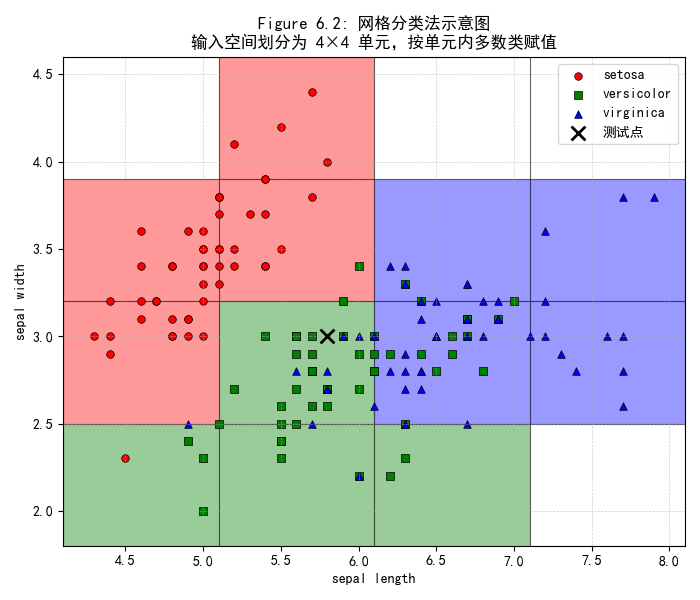
\includegraphics[width=0.3\textwidth]{fig62-iris-scatter.png}
\caption{分类的一种方法，对高维数据，方框的数量将急剧增加}
\label{fig:network}
\end{figure}


\end{frame}

% 第四部分：高维空间特性
\section{高维空间特性}
\begin{frame}{高维空间的几何直觉}
\begin{itemize}
    \item $D$维超球体体积：$V_D(r) = K_D r^D$
    $$V_1(r)=r, \quad V_2(r)=\pi r{\,}^2, \quad V_3(r)=\frac{4}{3}\pi r{\,}^3.$$

    \item 计算四维超球体的体积和表面积。

    \item 半径 $1-\epsilon$ 到 $1$ 之间的体积比例：
    \begin{align*}
        \frac{V_D(1) - V_D(1 - \epsilon)}{V_D(1)} = 1 - (1 - \epsilon)^D
    \end{align*}
    
    \item 在高维空间中，超球体的大部分体积集中在表面附近的薄壳中！
\end{itemize}
\end{frame}

\begin{frame}{高维空间中的高斯分布}
\begin{itemize}
    \item 高维空间中高斯分布的概率质量也集中在特定半径的薄壳中
    \item 低维空间的几何直觉在高维空间中可能失效
    \item 高维空间也可能有优势：使原本线性不可分的问题变得线性可分
\end{itemize}

\begin{figure}
\centering
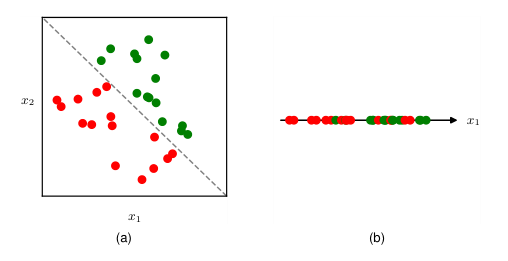
\includegraphics[width=0.4\textwidth]{fig66.png}
\caption{二维数据可分，一维数据不可分的例子}
\label{fig:6-6}
\end{figure}

\end{frame}

% 第五部分：数据流形
\section{数据流形}
\begin{frame}{数据流形}
\begin{itemize}
    \item 实际数据通常被限制在具有较低有效维度的数据空间区域中。
    \item 图像示例：尽管图像像素定义了高维空间，但实际图像位于三维流形上。
    \item 流形通常是高度非线性的。
\end{itemize}

\begin{figure}
\centering
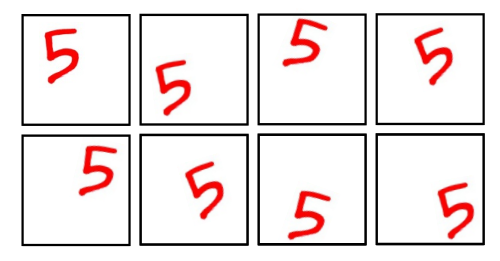
\includegraphics[width=0.4\textwidth]{fig67.png}
\caption{这些图像之间的区别只有旋转和平移，因此它们都存在于高维空间的一个三维流形上。}
\label{fig:6-7}
\end{figure}

\end{frame}

\begin{frame}{径向基函数与支持向量机}
\begin{itemize}
    \item 径向基函数 (RBF)：
    \begin{align*}
        \phi_n(\mathbf{x}) = \exp\left( -\frac{\|\mathbf{x} - \mathbf{x}_n\|^2}{s^2} \right)
    \end{align*}
    
    \item 支持向量机 (SVM)：自动选择基函数子集
    \item 缺点：计算复杂度高，不产生概率输出，难以扩展到多类问题
\end{itemize}
\end{frame}

% 第六部分：数据相关基函数
\section{数据相关基函数}
\begin{frame}{数据相关基函数}
\begin{itemize}
    \item 传统方法：专家知识手工设计特征
    \item 现代方法：从训练数据中学习基函数（领域知识更多体现在网络架构定性设计层面）
    \item 深度神经网络能够学习适应数据流形的基函数
    \item 能够学习深层层次表示
\end{itemize}
\end{frame}

\begin{frame}{自然图像 vs 随机图像}
\begin{itemize}
    \item 自然图像与随机图像示例展示了真实数据的强相关性
    \item 相邻像素在自然图像中具有相似的颜色
    \item 自然图像仅覆盖高维空间的一小部分
\end{itemize}
\end{frame}

% 总结
\begin{frame}{总结}
\begin{itemize}
    \item 固定基函数在高维空间中面临严重挑战
    \item 维度诅咒导致模型效率低下
    \item 数据流形概念解释了高维数据的有效低维结构
    \item 需要数据相关的、自适应的基函数
    \item 深度神经网络提供了有效的解决方案
\end{itemize}
\end{frame}

\end{document}